\documentclass[11pt,a4paper]{article}

\usepackage[utf8]{inputenc}
\usepackage[T1]{fontenc}
\usepackage[spanish]{babel}
\usepackage{amsmath,amssymb,bm}
\usepackage{booktabs}
\usepackage{graphicx}
\usepackage{geometry}
\usepackage{hyperref}
\geometry{margin=2.25cm}
\graphicspath{{figures/}}

\title{Auditoría FOM de la estabilidad tangente de la energía del RVE}
\author{Experimento reproducible para la PANN con simetría $D_4$}
\date{\today}

\begin{document}
\maketitle

\begin{abstract}
Antes de decidir si una PANN debe imponer una tangente definida positiva, se
mide esa propiedad directamente en el modelo de orden completo (FOM). El
resultado es inequívoco dentro de la envolvente de datos actual: la Hessiana de
la energía es positiva definida en la referencia y en un estado comprimido,
pero tiene autovalores negativos en estados mixtos, de gran tracción y en un
estado estrictamente reservado de Stage--10. Por tanto, imponer globalmente
$\bm D_E\succ0$ haría que el surrogate contradijese al FOM en parte del dominio
de interés. Esta conclusión se ha comprobado con dos pasos de diferencias
finitas.
\end{abstract}

\section{Pregunta que se mide}

El objetivo no es evaluar una red neuronal ni un HPROM. Se mide solamente la
energía macroscópica que resulta de resolver el RVE completo. Se usa la
convención ya empleada por la PANN:
\begin{equation}
 \bm e=[E_{11},E_{22},\gamma_{12}]^T,
 \qquad \gamma_{12}=2E_{12}.
\end{equation}
La energía directa del RVE se denota por $W(\bm e)$. La tensión conjugada a
esta convención es
\begin{equation}
 \bm s=\frac{\partial W}{\partial \bm e}
 =[S_{11},S_{22},S_{12}]^T,
\end{equation}
y la matriz pertinente para la pregunta del profesor es
\begin{equation}
 \bm D_E=\frac{\partial\bm s}{\partial\bm e}
 =\frac{\partial^2W}{\partial\bm e^2}.
 \label{eq:tangent}
\end{equation}

Al provenir de una energía dos veces diferenciable, $\bm D_E$ es simétrica. La
hipótesis adicional de convexidad estricta en $E$ sería
\begin{equation}
 \bm v^T\bm D_E(\bm e)\bm v>0
 \qquad\text{para todo }\bm v\neq\bm0.
 \label{eq:spd}
\end{equation}
Es importante no confundir \eqref{eq:tangent} con una derivada de tensión de
Cauchy. A gran deformación,
\begin{equation}
 \bm\sigma=J^{-1}\bm F\bm S\bm F^T,
\end{equation}
de modo que $\partial\bm\sigma/\partial\bm E$ contiene también términos
geométricos y no es la Hessiana de $W$. Este informe responde específicamente a
la condición de convexidad usada por una PANN con entrada $E$ o $C$.

\section{Medición directa con el FOM}

Se seleccionaron seis estados convergidos: dos cercanos a regímenes estables,
tres de gran deformación en las trayectorias Stage--1 y uno estrictamente
reservado de Stage--10. Cada estado base se toma de la historia de
desplazamientos FOM ya convergida. Desde él se resuelven de nuevo, por
continuación, los 18 estados de un stencil central alrededor de $\bm e_0$.
No se usa ninguna predicción PANN, ICNN, ICKAN, PROM o HPROM.

En cada punto perturbado se evalúa directamente la densidad de energía
Neo--Hookeana microscópica en los puntos de Gauss convergidos y se promedia en
el volumen de referencia. Para una componente $i$ y un paso $h$, por ejemplo,
\begin{equation}
 [\bm D_E]_{ii}\simeq
 \frac{W(\bm e_0+h\bm e_i)-2W(\bm e_0)+W(\bm e_0-h\bm e_i)}{h^2},
\end{equation}
y para $i\neq j$,
\begin{equation}
 [\bm D_E]_{ij}\simeq
 \frac{W_{++}-W_{+-}-W_{-+}+W_{--}}{4h^2}.
 \label{eq:mixed}
\end{equation}
Aquí $W_{ab}=W(\bm e_0+a h\bm e_i+b h\bm e_j)$, con $a,b\in\{-1,1\}$.
El stencil tiene por tanto $1+6+12=19$ valores de energía por estado. El paso
principal es $h=10^{-2}$.

La derivada central de la energía también reproduce las tensiones directas
almacenadas, con discrepancias del orden de $10^{-5}$ relativo en los estados
tensiles no nulos. Esto verifica que el cálculo está usando la misma energía y
la misma convención de trabajo que la PANN.

\section{Resultados}

La Figura~\ref{fig:eigs} muestra los autovalores de la matriz medida. La
Figura~\ref{fig:matrices} muestra las matrices completas en GPa; la simetría
de cada matriz es consecuencia de haber derivado una única energía escalar.

\begin{figure}[htbp]
 \centering
 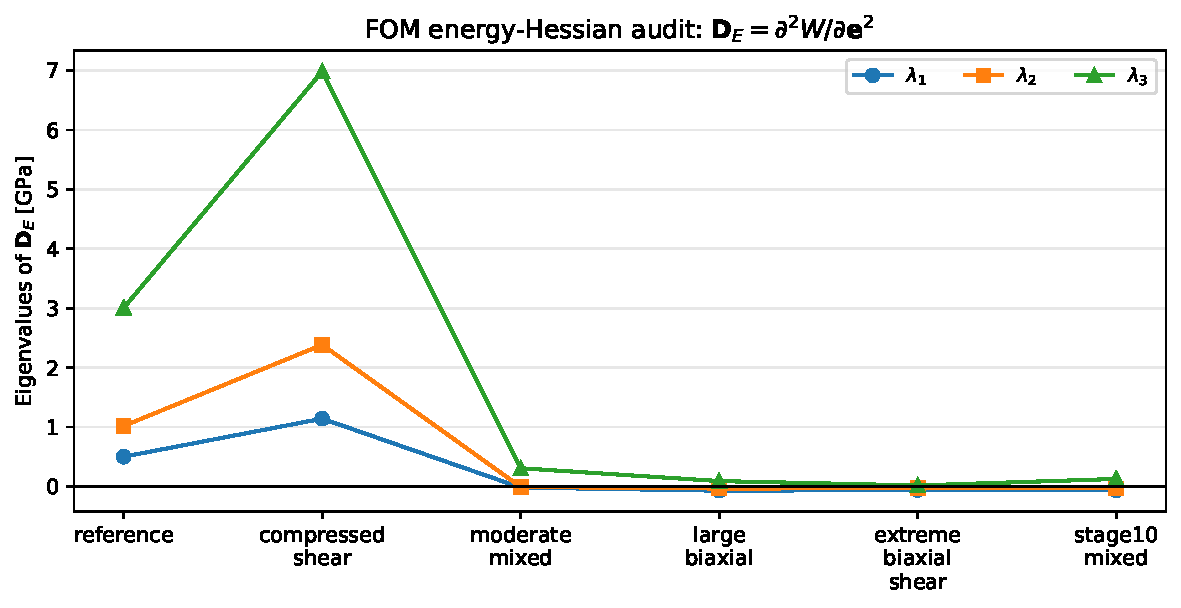
\includegraphics[width=0.95\linewidth]{fom_tangent_eigenvalues.pdf}
 \caption{Autovalores de $\bm D_E=\partial^2W/\partial\bm e^2$ medidos con el
 FOM. La línea horizontal marca el límite de positividad.}
 \label{fig:eigs}
\end{figure}

\begin{table}[htbp]
 \centering
 \small
 \begin{tabular}{l c c c}
\toprule
State & $[E_{11},E_{22},\gamma_{12}]$ & eigenvalues of $\mathbf{D}_E$ [GPa] & SPD? \\
\midrule
reference & $[0, 0, 0]$ & $[0.50167, 1.0193, 3.0055]$ & yes \\
compressed\_shear & $[-0.1, -0.1, 0.1]$ & $[1.1422, 2.3852, 6.9836]$ & yes \\
moderate\_mixed & $[0.5, 0.5, 0.05]$ & $[-0.017159, -0.007317, 0.30795]$ & no \\
large\_biaxial & $[1, 1, 0]$ & $[-0.069526, -0.033408, 0.091833]$ & no \\
extreme\_biaxial\_shear & $[2, 2, 0.1]$ & $[-0.059013, -0.028513, 0.017463]$ & no \\
stage10\_mixed & $[0.8857, 0.8, 0.04286]$ & $[-0.064801, -0.031075, 0.12804]$ & no \\
\bottomrule
\end{tabular}

 \caption{Estados FOM auditados. Un único autovalor negativo es suficiente para
 refutar $\bm D_E\succ0$ globalmente en la envolvente considerada.}
 \label{tab:results}
\end{table}

\begin{figure}[htbp]
 \centering
 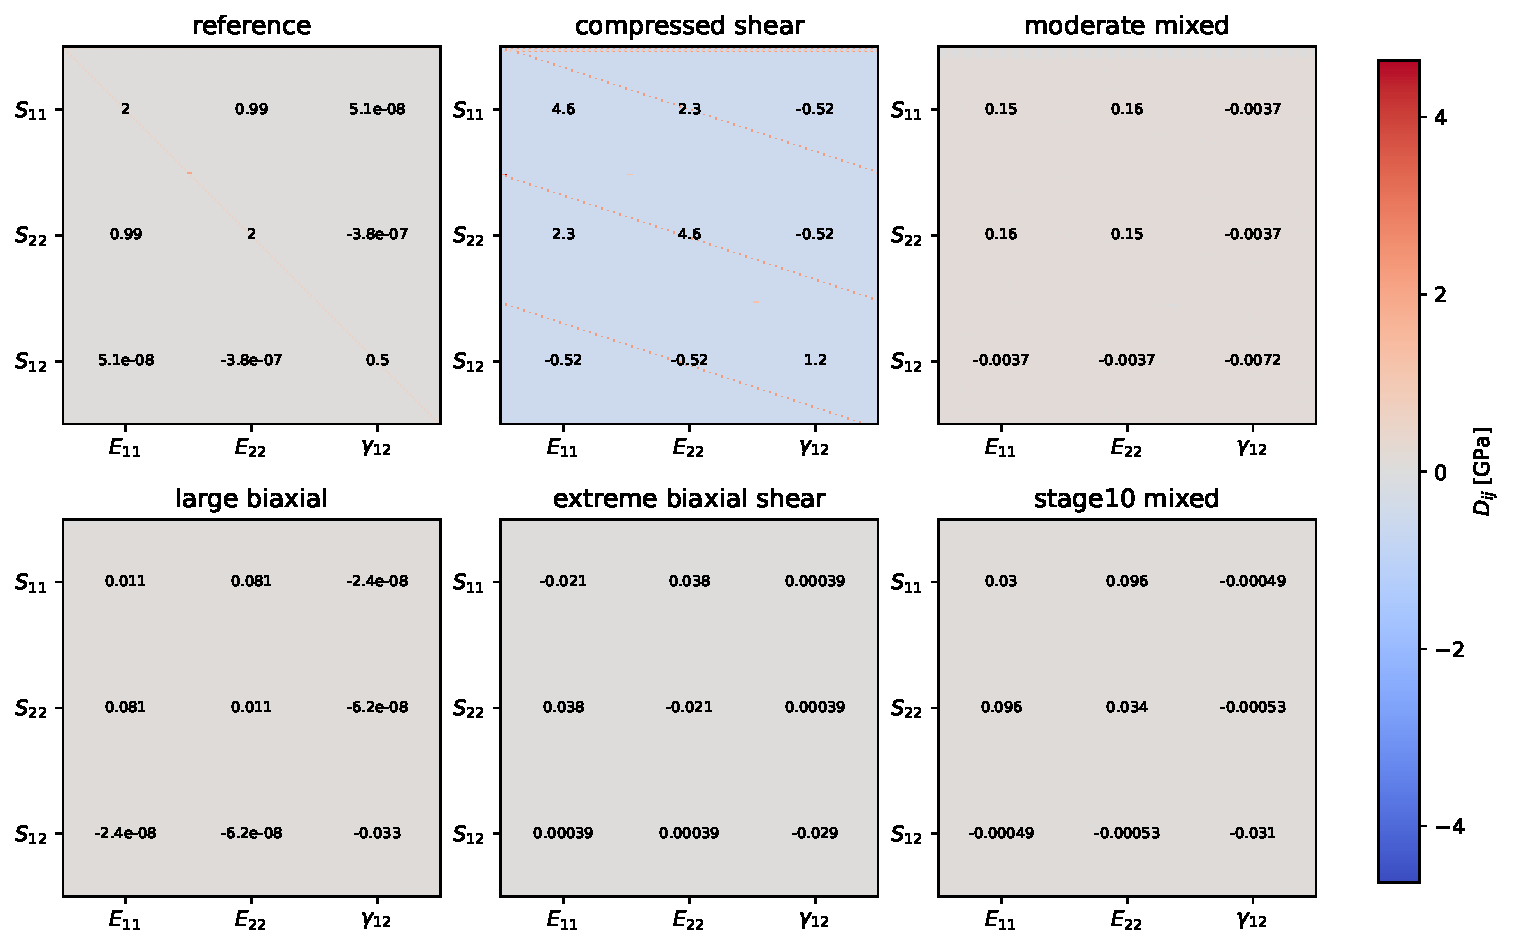
\includegraphics[width=0.98\linewidth]{fom_tangent_matrices.pdf}
 \caption{Matrices tangentes medidas, en GPa. Las dos direcciones normales se
 acoplan fuertemente; la indefinitud no se debe a una falta de simetría
 numérica.}
 \label{fig:matrices}
\end{figure}

La pérdida de positividad no es marginal ni se limita a una trayectoria de
entrenamiento. En particular, el estado Stage--10
\begin{equation}
 [E_{11},E_{22},\gamma_{12}]
 =[0.885714,\,0.800000,\,0.042857]
\end{equation}
tiene $\lambda_{\min}(\bm D_E)=-0.0648006\,\mathrm{GPa}$. Es un estado
admisible: los autovalores de su tensor $\bm C$ son positivos
($2.590$ y $2.782$). Por tanto, el autovalor negativo no procede de acercarse a
$J=0$ ni de una configuración no física.

\section{Comprobación del paso de diferencias finitas}

Los dos estados más relevantes se repitieron con $h=5\times10^{-3}$. La
variación relativa de $\lambda_{\min}$ es de solo unos pocos $10^{-6}$, mientras
que los autovalores negativos permanecen del orden de $10^{-2}\,\mathrm{GPa}$.
La señal no es, por tanto, un artefacto de truncamiento de las diferencias
finitas.

\begin{table}[htbp]
 \centering
 \small
 \begin{tabular}{l c c c}
\toprule
State & $h$ & $\lambda_{\min}(\mathbf{D}_E)$ [GPa] & relative change \\
\midrule
extreme\_biaxial\_shear & 0.01 & -0.05901254 & -- \\
 & 0.005 & -0.05901237 & 3.01e-06 \\
stage10\_mixed & 0.01 & -0.06480063 & -- \\
 & 0.005 & -0.06480048 & 2.24e-06 \\
\bottomrule
\end{tabular}

 \caption{Sensibilidad al paso.}
\end{table}

\section{Conclusión para la arquitectura}

La evidencia FOM permite tomar una decisión clara:
\begin{itemize}
 \item No es correcto imponer globalmente $\bm D_E\succ0$ sobre el dominio
 actual de entrenamiento y Stage--10. Cuatro de los seis estados FOM
 medidos violan esa condición.
 \item Una ICNN convexa en $E$ sería una aproximación deliberadamente más
 restrictiva que el FOM. Puede ser útil como baseline o como modelo local cerca
 de la referencia, pero no debe presentarse como la física exacta del RVE en
 toda esta envolvente.
 \item Esta observación \emph{no} refuta la policovexidad. La convexidad en
 $E$ y la policovexidad en $(\bm F,\operatorname{cof}\bm F,J)$ son condiciones
 diferentes: una energía policovexa puede tener una Hessiana indefinida al
 parametrizarla por $E$.
 \item Si se desea usar una penalización SPD en una loss, debe formularse como
 una regularización local y muestreada, no como una condición global que el FOM
 no satisface.
\end{itemize}

En consecuencia, la siguiente arquitectura de invariantes $D_4$ debe evaluarse
primero por simetría, objetividad, energía--tensión y precisión. La elección
entre una PANN libre, una ICNN en $E$ y una PANN policovexa debe reportar
explícitamente este compromiso entre fidelidad y garantía matemática.

\end{document}
